\label{sim_analysis}

Upon completion of each simulation run, the saved data files were analyzed to determine the regions of the simulation which had melted.  This was done by developing a map which marked the locations of the domain that had ever been in the fluid phase.  This map was then used to determine the width and depth of the melt track along the scan length, excluding the beginning and end where effects from starting and stopping motion would affect the results.  These width and depth measurements along the scan length were averaged to develop a single measurement which could be compared to experimentation.  

The experimental results were similarly determined, however instead of a continuous set of measurements, there were 4 discrete measurements.  These were obtained by slicing the substrate at the prescribed locations using a wire \ac{EDM}.  These slices were polished and etched in order to make the microstructural differences visible, an example of this can be seen in Figure \ref{fig:7075_7_8C}, where the dark region had been melted during the experimentation.
\begin{figure}[!htb]
	\centering
	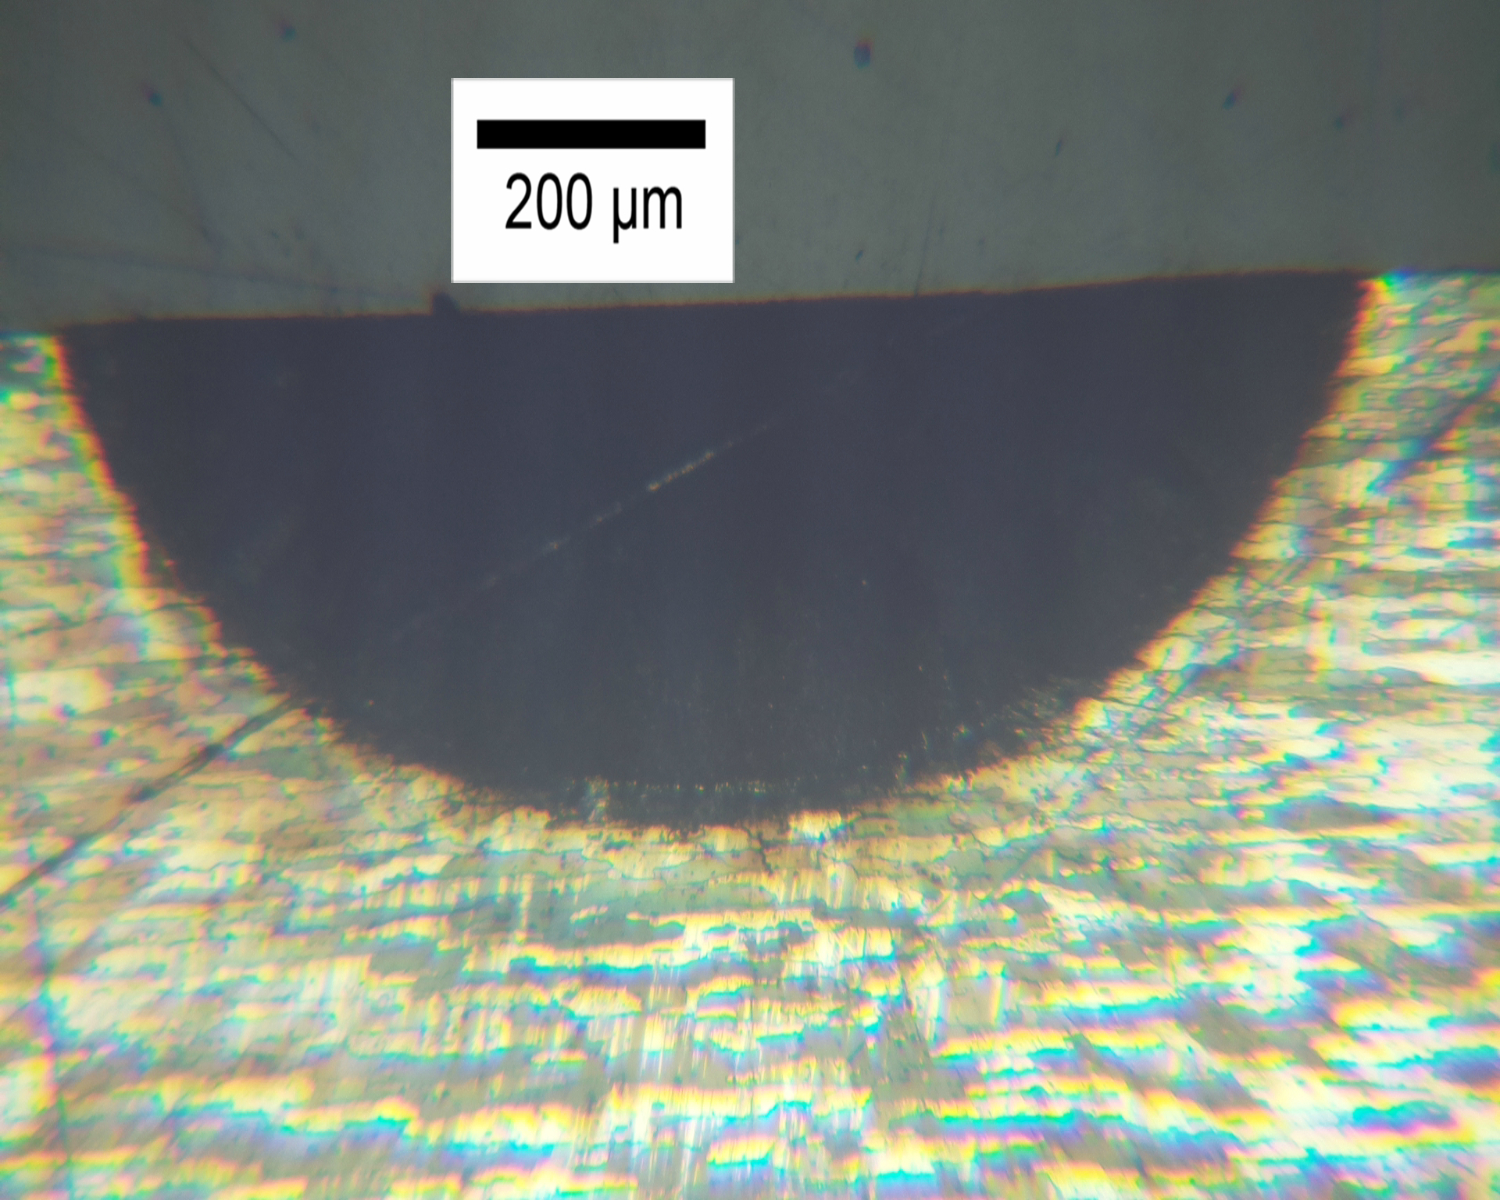
\includegraphics[width=0.5\textwidth]{7075_7_8C}
	\caption{Example of sliced, polished, and etched slice from experimentation}
	\label{fig:7075_7_8C}
\end{figure}

In order for the Nelder-Mead search to function properly, a response variable needed to be defined.  This function needed to characterize the accuracy of the simulation into a single parameter which could be minimized and upon minimization would result in the most accurate simulation.  To accomplish this goal, Equation \ref{eqn:response} was developed.  This equation takes into account the error in the width of the simulation along with the error in the depth.  This equation results in a non-negative number where 0 represents a simulation which perfectly matched experimentation.

\begin{equation}\label{eqn:response}
	\begin{split}
		Response =  \Biggl ( &\frac{\lvert Sim.\ Width - Exp.\ Width \rvert}{Exp.\ Width} + \\ 
		&\frac{\lvert Sim.\ Depth - Exp.\ Depth \rvert}{Exp.\ Depth} \Biggr ) * 100
	\end{split}
\end{equation}